\documentclass[twocolumn]{rbef}
\usepackage{lipsum}
\usepackage[brazil]{babel}
\usepackage{color}% Allows color text
\usepackage{ulem}% allows strike-out using sout

\newif\ifcmnt
%  Use \cmntfalse to not see comments when it is latex'ed
% \cmntfalse
%  Use \cmnttrue to see the comments
\cmnttrue 
\ifcmnt
    \providecommand{\aucmnt}[1]{#1}
    \providecommand{\editcolor}[2]{\textcolor{#1}{#2}}
\else
    \providecommand{\aucmnt}[1]{}
    \providecommand{\editcolor}[2]{#2}
\fi
\newcommand{\HV}[1]{\editcolor{blue}{#1}}
\newcommand{\HVc}[1]{\aucmnt{\editcolor{blue}{[HV: #1]}}}
\newcommand{\HVs}[1]{\aucmnt{\editcolor{blue}{\sout{#1}}}}
\newcommand{\SG}[1]{\editcolor{magenta}{#1}}
\newcommand{\SGs}[1]{\aucmnt{\editcolor{magenta}{\sout{#1}}}}
\newcommand{\SGc}[1]{\aucmnt{\editcolor{magenta}{[SG: #1]}}}
\newcommand{\LS}[1]{\editcolor{green}{#1}}
\newcommand{\LSs}[1]{\aucmnt{\editcolor{green}{\sout{#1}}}}
\newcommand{\LSc}[1]{\aucmnt{\editcolor{green}{[LS: #1]}}}
% find more colors at https://en.wikibooks.org/wiki/LaTeX/Colors#The_68_standard_colors_known_to_dvips



\titulocabecalho{A Computational Toolbox for Teaching Quantum Mechanics and Quantum Optics}
\autorcabecalho{J. L. E. Silva, S. Glancy, H. M. Vasconcelos}

\numeracao{xxxx}
\volume{xx}
\numero{xx}
\ano{2010xx}
\doi{http://dx.doi.org/xxxx}
\tipodeartigo{Artigos Gerais}
%\addtocounter{page}{566} %% \setcounter produces extra white page!!! use ===\addtocounter===





        \author[1]{Silva, J. L. E.} 
        \author[2]{Glancy, S.}
        \author[1,2]{Vasconcelos, H. M.}
        \affil[1]{Departamento de Engenharia de Teleinformática, Universidade Federal do Ceará, Fortaleza, CE, Brazil\thanks{\href{emailto:fulano@ferro.com}{hilma@ufc.br}}
                } 
                \affil[2]{Applied and Computational Mathematics
                  Division, National Institute of Standards and Technology, Boulder, CO, USA}


\titulo{A Computational Toolbox for Teaching Quantum Mechanics and Quantum Optics}

\subtitulo{Uma Ferramenta Computational para o Ensino da Mecânica Quântica e da Óptica Quântica}

%++++++++++++++++++++++++++++++++++++++++++++++++++



%++++++++++++++++++++++++++++++++++++++++++++++++++




\begin{document}
        

\begin{primeirapagina}


%\begin{center}
%\vspace{-12pt}
%\small{Recebido em xxx. Aceito em xxx}
%\end{center}


        \begin{abstract}
          We describe a collection of code\SGs{s} that \SGs{may
            be}\SG{are} useful in teaching of quantum mechanics and
          quantum optics courses. The toolbox has been developed using
          Matlab programming language, but we expect that a
          translation to an open source mathematics software could be
          easily done \SGc{Want to ask Italo to do this?}. These codes
          can be used to help visualize quantum states of light using
          Wigner function, how these states may be affected by loss,
          among other things.  \keywords{Quantum states of light,
            Wigner function, purity, fidelity.}

        \end{abstract}

        
        \begin{otherlanguage}{english}
        

        \begin{abstract}
Descrevemos um conjunto de códigos computacionais que podem ser úteis no ensino da
mecânica quântica e da óptica quântica. Esse ferramental foi desenvolvido usando a
linguagem de programação Matlab, mas esperamos que uma tradução desses códigos para 
uma linguagem de software aberto possa ser feito facilmente. Os códigos aqui descritos
ajudam a visualizar estados quânticos da luz usando a função de Wigner, como estes
estados podem ser afetados por perdas, entre outras coisas.
        \palavraschave{Estados quânticos da luz, função de Wigner, pureza, fidelidade.}
        
        \end{abstract}
        \end{otherlanguage}

        \end{primeirapagina}
\saythanks

\section{Introduction}
Quantum mechanics is one of the most crucial, and yet, challenging, topics of modern physics~\cite{Matthews, Baily2010}. With its application to many and important technological problems, the challenges in teaching quantum mechanics are now part not only of the physical science undergraduate curricula, but also of engineering education, especially in the area of communications~\cite{Mermin2003, Grau2004}. Some of the challenges are also faced by professors when teaching quantum optics in a graduate (or undergraduate) level. Any visualization tools in these areas of knowledge can be of great assistance towards an appropriated grasp of concepts by students~\cite{Singh2008, McKagan2008, Gong2015, Tomandl2015, Kohnle2015}. 

We \SGs{are going to} describe here a set of codes developed using
Matlab programming language and their use to give insight into the
nature of quantum mechanics and quantum optics. In the context of our
work, we use a formulation of quantum mechanics that is equivalent to
the standard \SG{pedagogical} approach: the Wigner
function~\cite{Case2008}.

If the wave function $\psi(x)$ of a system is known, we may easily determine the probability density $|\psi(x)|^2$ in position space $x$. On the other hand, the momentum distribution, $|\phi(p)|^2$, is difficult to visualize if we have only $\psi(x)$. That is the standard formulation of quantum mechanics. We may alternatively approach quantum mechanics through a function that displays the probability distribution simultaneously in the $x$ and $p$ variables. This function was introduced in 1932 by Eugene Wigner~\cite{Wigner1932} and is defined as:
\begin{eqnarray}
W(x,p) = \frac{1}{h} \int e^{-i p y/\hbar} \psi(x+y/2) \psi^{\ast}(x-y/2) dy.
\label{eq-Wigner}
\end{eqnarray}
Quantum mechanical probability densities in position space $x$ and momentum space $p$ can be obtained from the marginals of the Wigner function, since
\begin{eqnarray}
&&\int W(x,p) dp = \psi^{\ast}(x) \psi(x) = |\psi(x)|^2, \nonumber \\
&&\int W(x,p) dx = \phi^{\ast}(p) \phi(p) = |\phi(p)|^2.
\end{eqnarray}
The Wigner function $W(x, p)$ is known as a quasi\SG{-}probability
\SGs{function}\SG{distribution} because, even though it is real and
normalized to one, \SGs{it is not necessarily non-negative}\SG{for
  some states it is negative over some of $(x,p)$ space. The amount of
  negativity is a measure of the ``nonclassicality'' of a
  state.[citation needed]}

This paper is organized as follows: in Section~\ref{harmonic-oscillator} we describe the use of the computational toolbox to study the harmonic oscillator. In Section~\ref{other-states} we show the use of the visualization toolbox for other states of the light, and in Section~\ref{conclusion} we make some concluding remarks.

\section{Example: simple harmonic oscillator \SG{Fock states}}
\label{harmonic-oscillator}
We can use the wave function for each energy state of the harmonic
oscillator and Eq.~(\ref{eq-Wigner}) to find the corresponding Wigner
function for each of these states. Alternatively, we may use the
Algebraic Method described in~\cite{Griffiths2004}, \SGc{Something is
  wrong with this sentence, and I'm not sure what it is trying to
  say.} continue the discussion to introduce the number operator,
$\hat{n} = \hat{a}^{\dagger}\hat{a}$, and the ket notation for the
harmonic oscillator's eigenstates $|n\rangle$, as done
in~\cite{Sakurai1993}. \SGc{I would explain that the code represents
  the states in the photon number basis here.  Also why we need to
  specify the maximum number of photons and how to choose the maximum
  number.}

In the toolbox, there is a routine for generating the pure state vector for photon number eigenstate $n$ in the photon number basis, as show bellow. When calling this routine, the students need to specify two variables: the number of photons, $n$, and the photon number at which the Hilbert space is truncated \SGs{(since the routines where developed to study Quantum State Tomography, we need to specify where we truncate the Hilbert space)}.
\begin{figure}[h]
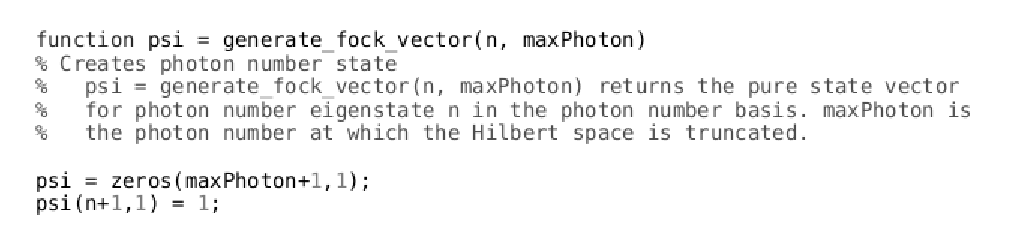
\includegraphics[width=0.5\textwidth]{generate_fock_vector1.eps}
\end{figure}

\SGc{LaTeX has nice tools for inserting code into text.  Check out
  \url{https://en.wikibooks.org/wiki/LaTeX/Source_Code_Listings}.
  I think that will be easer to mannage than inserting the code as
  images.}

The following lines of code plot the Wigner function of a vacuum state ($n =0$). Notice that to plot the Wigner function of any $n$ photon state, all that we need to do is change the number of photons $n$ in the routine. The resulting plot for the vacuum state can be seen in Figure~\ref{fig-W-n=0}.
\begin{figure}[h]
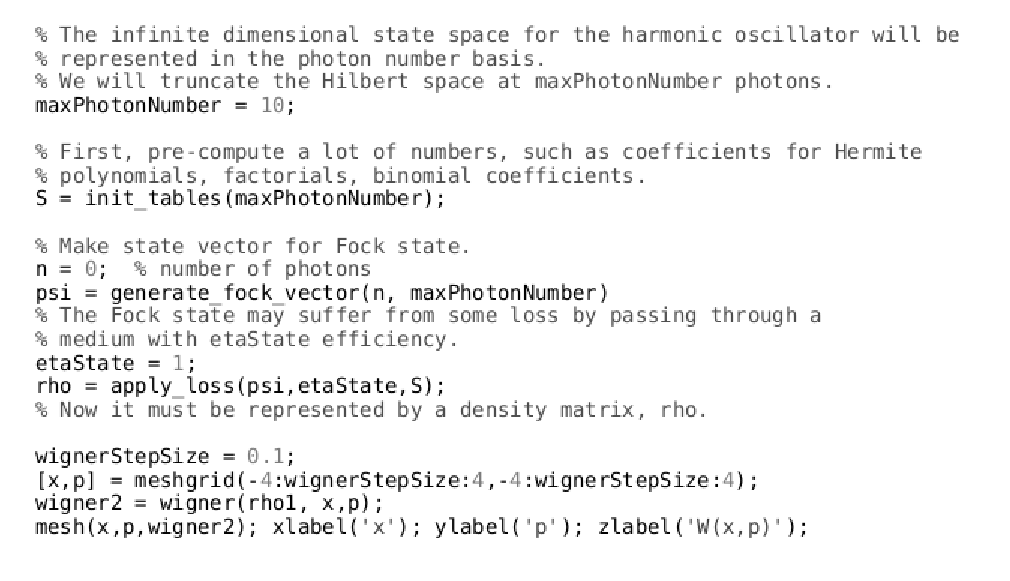
\includegraphics[width=0.5\textwidth]{generate_fock_vector2.eps}
\end{figure}
\SGc{I would remove the lines for \texttt{etaState = 1} and \texttt{rho = apply\_loss}
  because they are not used here and they add clutter.  Also, maybe
  we should write a graphing function that encapsulates the last four
  lines, gives a default step size, and draws the graph.}

\SGc{After introducing each figure, I recommend writing a few
  sentences about what features of the figure students should notice
  to increase their understanding of the state's properties.}
\begin{figure}[h]
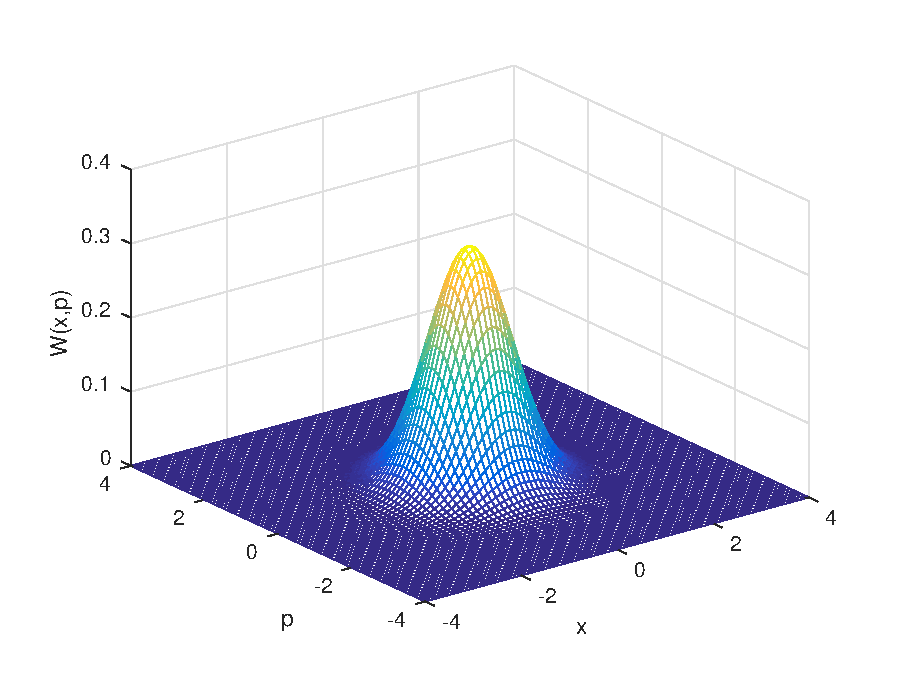
\includegraphics[width=0.5\textwidth]{fockn=0.eps}
\caption{Wigner function of a vacuum state $n=0$.}
\label{fig-W-n=0}
\end{figure}

Figure~\ref{fig-W-number4} shows the plot of $W(x,p)$ of a $n=4$
number state. \SGs{In here it can be seen}\SG{One can see} the negative part of the Wigner function, usually related to the nonclassicality of the state.
\begin{figure}[h]
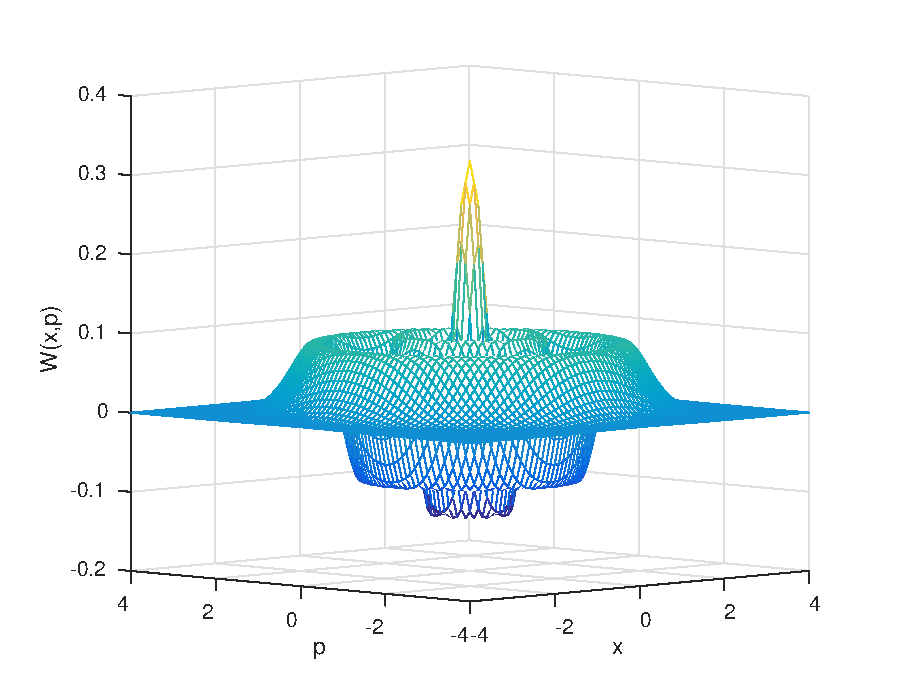
\includegraphics[width=0.5\textwidth]{fockn=4.eps}
\label{fig-W-number4}
\caption{Wigner function of a number state $n=4$.}
\end{figure}

\section{Example: other states of light}
\label{other-states}
In the context of a quantum optics course, it is natural to study other states of light, such as coherent and squeezed states. Moreover, these states may also be introduced in an upperlevel quantum mechanics course. A coherent state is an eigenstate of the annihilation operator, $\hat{a}|\alpha\rangle = \alpha |\alpha\rangle$, where $\alpha$ is a complex number. Coherent states are minimum uncertainty states.

A squeezed state is a state of light where fluctuations are reduced below the standard quantum limit in one quadrature at the expense of increased fluctuations in the conjugate quadrature. The toolbox provides routines to generate a coherent and a squeezed vacuum state, as shown bellow.
\begin{figure}[h]
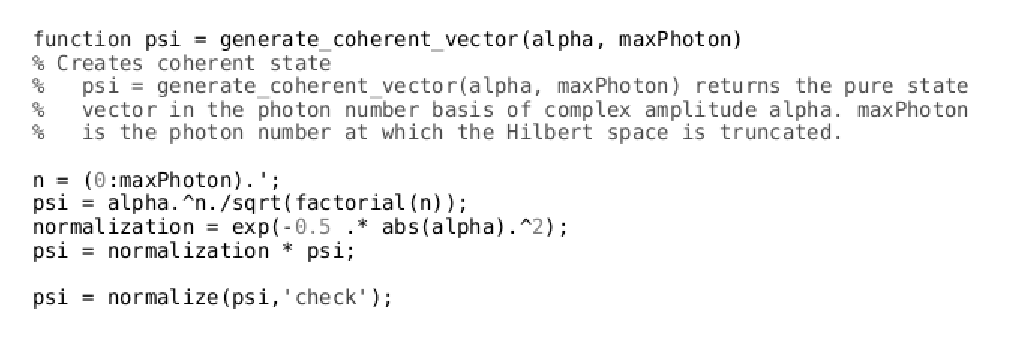
\includegraphics[width=0.5\textwidth]{generate_coherent_vector.eps}
\end{figure}
 
\begin{figure}[h]
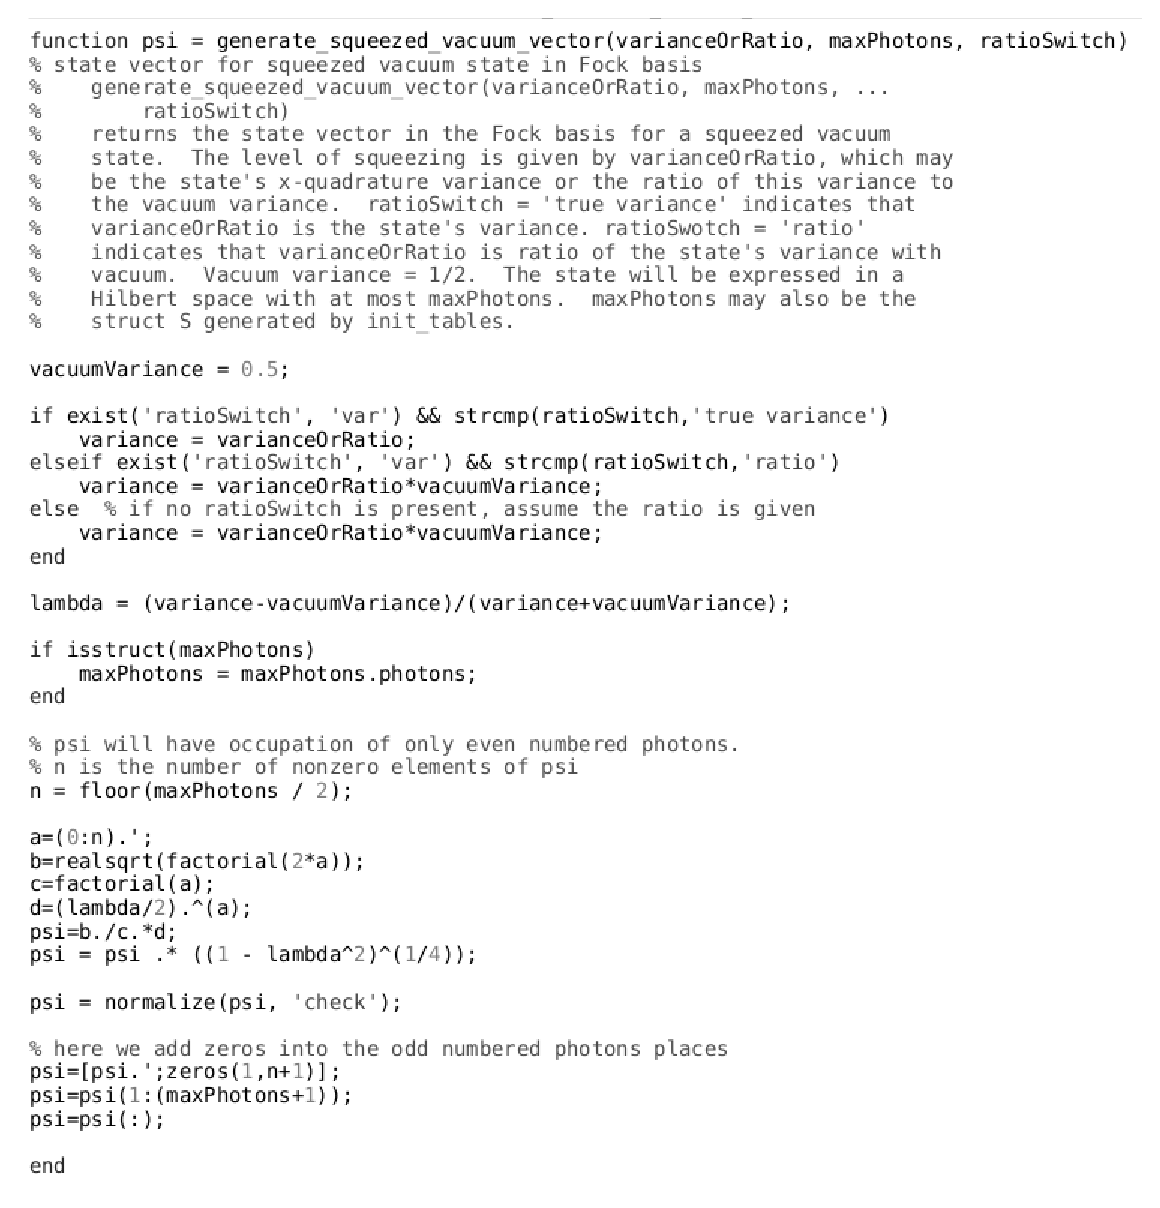
\includegraphics[width=0.5\textwidth]{generate_squeezed_vacuum_vector.eps}
\end{figure}
\SGc{I have always hated the \texttt{ratioSwitch} in
  \texttt{generate\_squeezed\_vacuum\_vector}.  It adds a lot of
  clutter here, so maybe we should remove it for this paper.}

To plot the Wigner function of a coherent state and a squeezed vacuum state, we use the lines of code showed. We may plot the Wigner function of coherent states of different amplitude by changing the value for $\alpha$ in the code. When plotting the Wigner function of a squeezed vacuum state, we need to specify if we are using the state's variance (as in the example showed) or the ratio of the state's variance with
respect to vacuum's variance (that is 1/2). Plotting different squeezed vacuum states is done by changing the variance or the ratio.

\begin{figure}[h!]
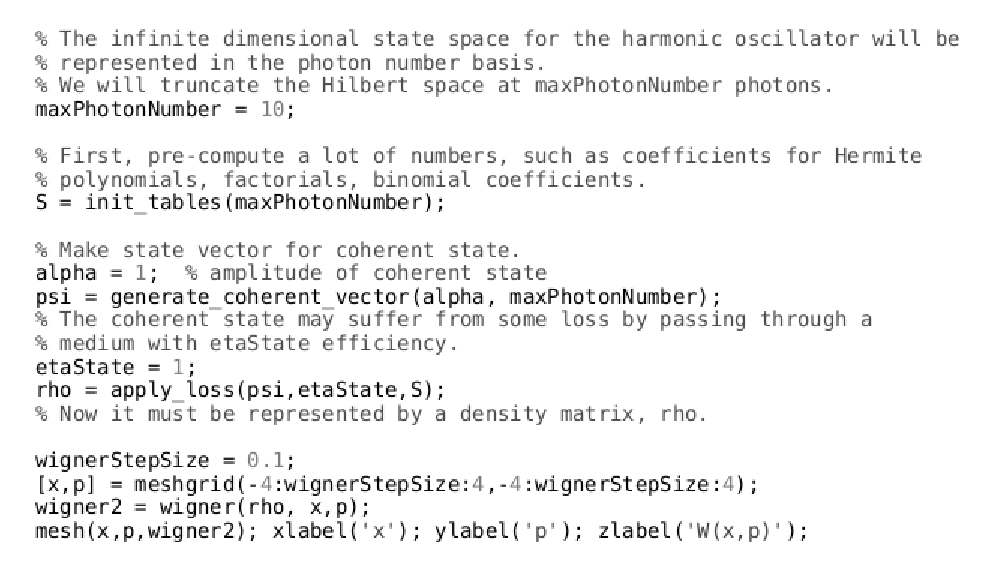
\includegraphics[width=0.5\textwidth]{wigner-coherent-alpha=1.eps}
\end{figure}
 
\begin{figure}[h!]
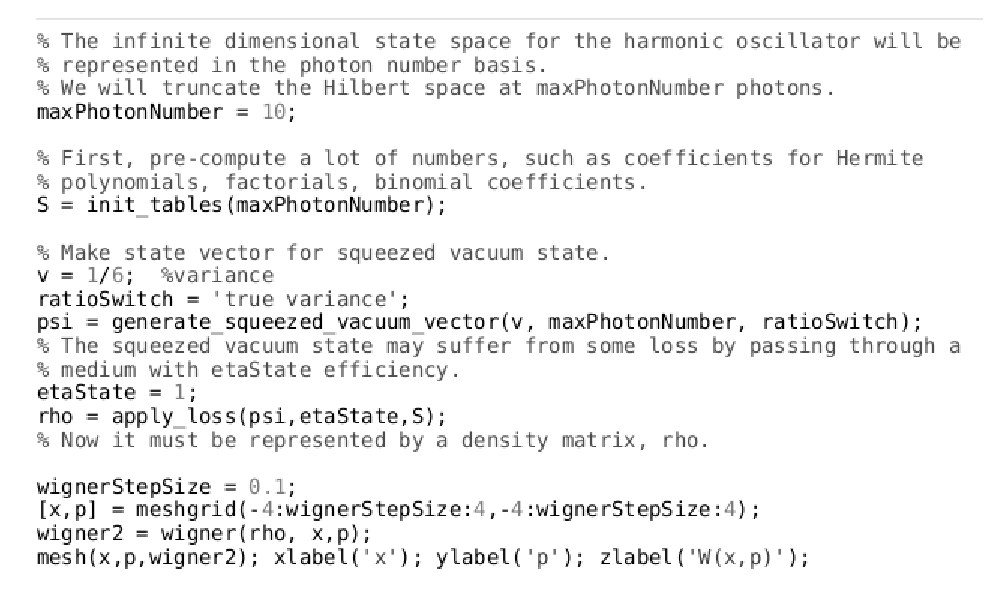
\includegraphics[width=0.5\textwidth]{wigner-squeezed.eps}
\end{figure}

In Figure~\ref{fig-coherent-alpha=1} we have the Wigner function of a coherent state with $\alpha = 1$. When students compare Figures~\ref{fig-W-n=0} and~\ref{fig-coherent-alpha=1}, they see that a coherent state is a displaced vacuum state. Figure~\ref{fig-squeezed-state} shows the Wigner function of a squeezed vacuum state with variance equals to 1/6 of vacuum variance.

\begin{figure}[h]
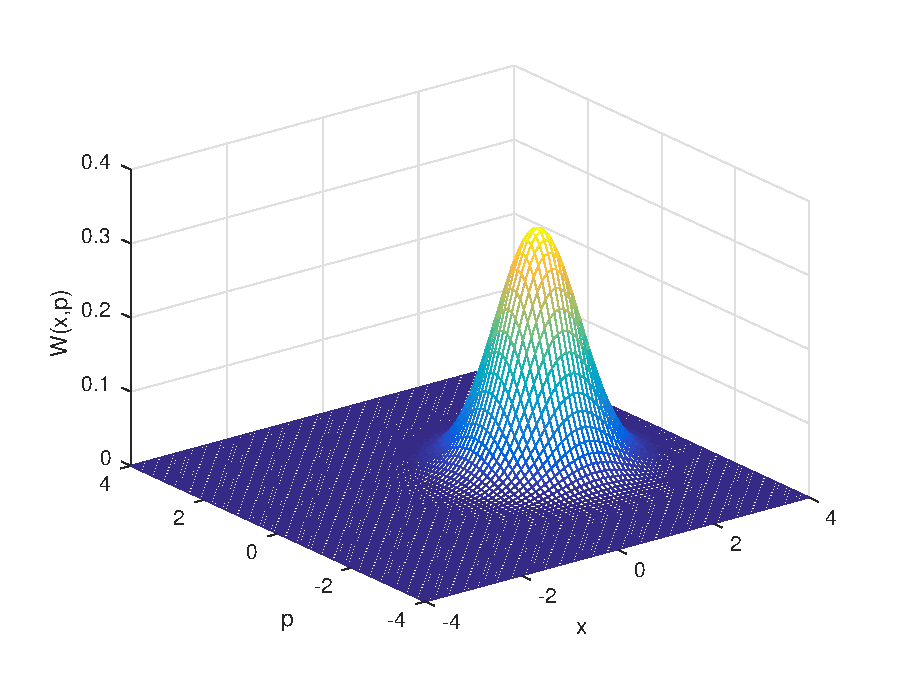
\includegraphics[width=0.5\textwidth]{coherent-alpha=1.eps}
\caption{Wigner function of a coherent state with $\alpha=1$.}
\label{fig-coherent-alpha=1}
\end{figure}

\SGc{I would not repeat the maxPhotonNumber and S assignments every time.}

\begin{figure}[h]
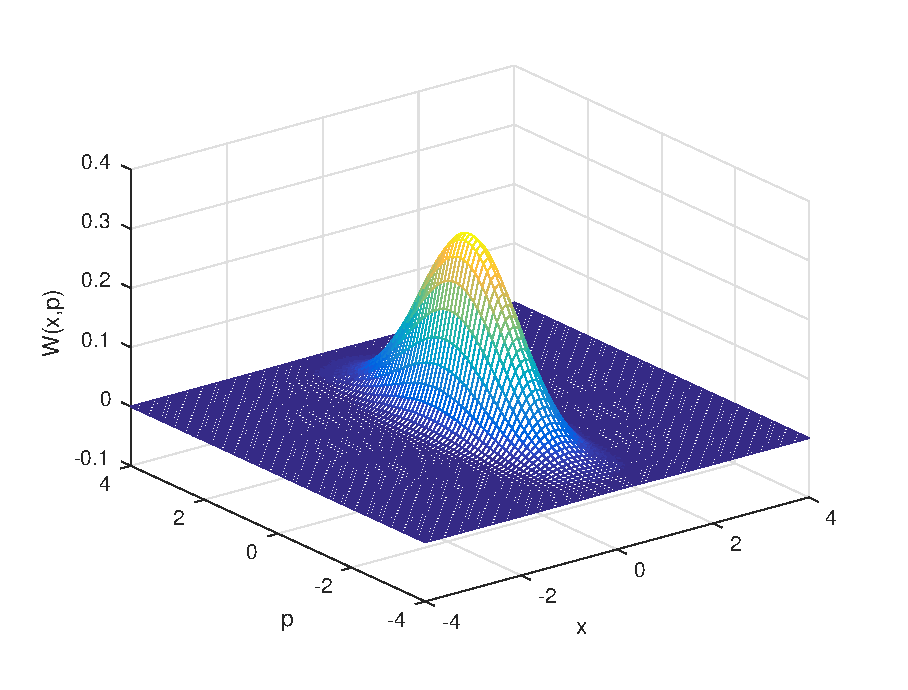
\includegraphics[width=0.5\textwidth]{wigner-squeezed1.eps}
\caption{Wigner function of a squeezed vacuum state with variance equals to 1/6 of vacuum variance.}
\label{fig-squeezed-state}
\end{figure}

Students from both courses \SGc{What are the two courses?} can explore the fundamental superposition principle of quantum mechanics using superpositions of coherent states, also known as Schr\"odinger cat states, such as:
\begin{eqnarray}
|\mathrm{cat}\rangle = \frac{1}{\sqrt{2\left( 1+ e^{-2|\alpha|^2} \cos \theta \right)}} \left(e^{i \theta} |-\alpha\rangle + |\alpha\rangle \right).
\end{eqnarray}
The routines to generate a cat state with amplitude $\alpha$ and to plot the corresponding Wigner function for such states are shown bellow. 
\begin{figure}[h!]
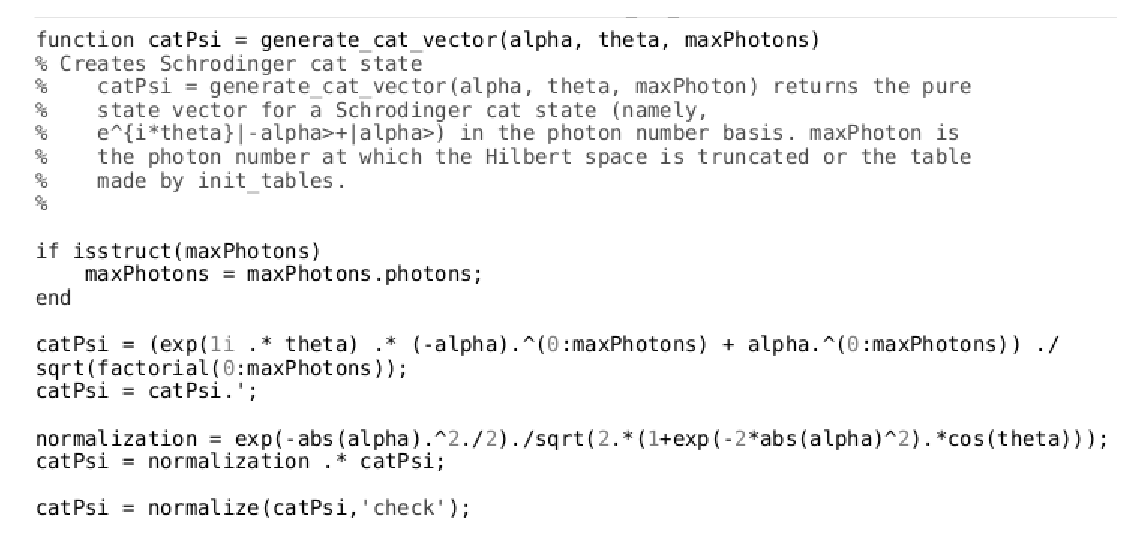
\includegraphics[width=0.5\textwidth]{generate_cat_vector.eps}
\end{figure}

\begin{figure}[h!]
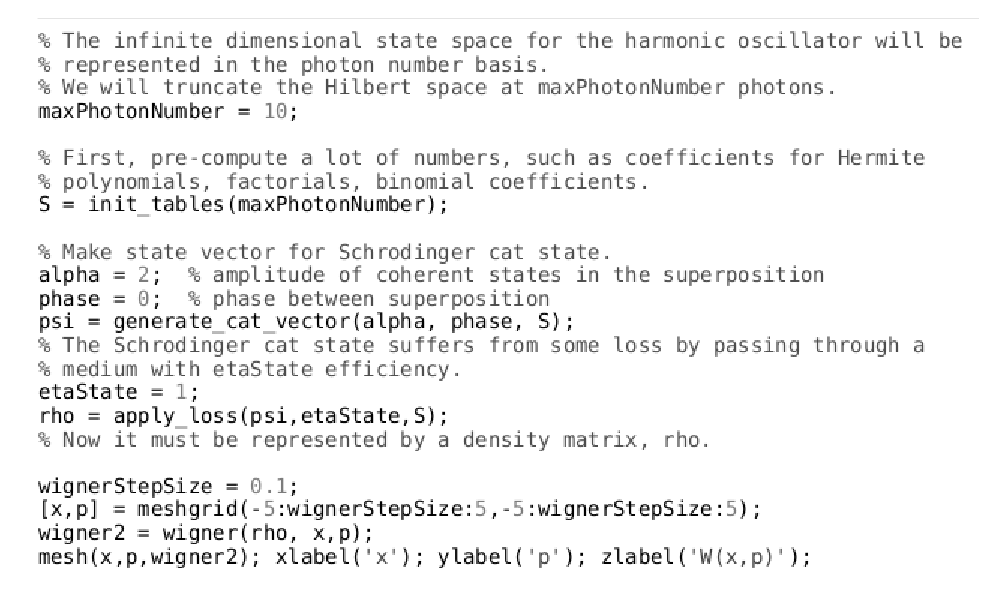
\includegraphics[width=0.5\textwidth]{wigner-cat.eps}
\end{figure}

Figure~\ref{fig-catstate} shows the Wigner function of a cat state with amplitude of coherent states in the superposition of $\alpha=2$ and superposition phase $\theta =0$. 

\begin{figure}[h]
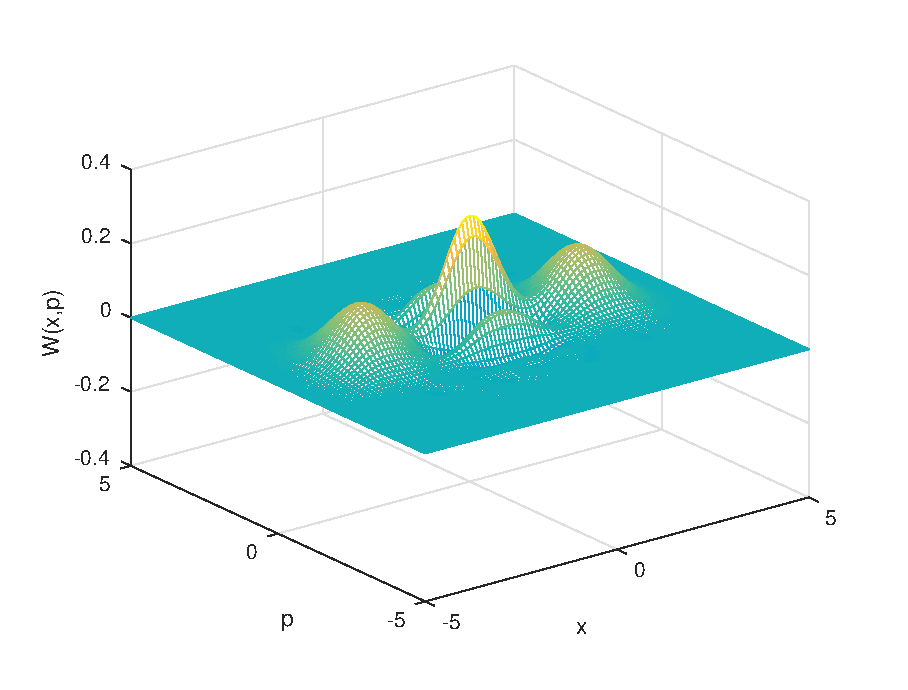
\includegraphics[width=0.5\textwidth]{wigner-cat-2.eps}
\caption{Wigner function of a cat state with amplitude of coherent states in the superposition $\alpha=2$ and superposition phase $\theta =0$.}
\label{fig-catstate}
\end{figure}

The effect of loss in any of the states shown here can be considered
and observed by changing the \texttt{etaState}. parameter when using
the lines of codes. Let us consider, for example, the effect of loss
in the cat state of Figure~\ref{fig-catstate}. For that, consider that
the state passed through a medium with 90 \% efficiency
(\texttt{etaState = 0.9}). The Wigner function for the state after the
loss is shown in figure~\ref{fig-catstate-loss}.  \SGc{Since we are
  now talking about mixed states, maybe we should explain how to
  calculate the Wigner function given a density matrix.}

\begin{figure}[h]
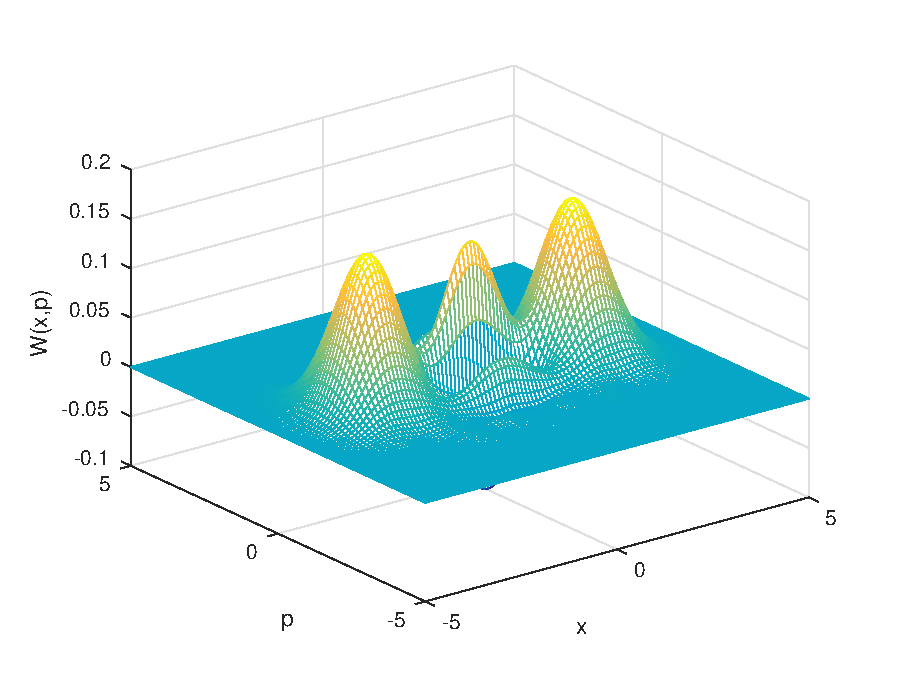
\includegraphics[width=0.5\textwidth]{wigner-cat-2-perda.eps}
\caption{Wigner function of a cat state with amplitude of coherent states in the superposition $\alpha=2$ and superposition phase $\theta =0$ after going through a medium with 90\% efficiency.}
\label{fig-catstate-loss}
\end{figure}

We then may use the following lines of code to calculate how "close" the state with loss is of the original state. That is done using the concept of fidelity, defined, for any two density matrices, $\rho$ and $\sigma$, as
\begin{eqnarray}
F(\rho,\sigma) = \left( Tr \left(\sqrt{\sqrt{\rho} \sigma \sqrt{\rho}}\right) \right)^2,
\end{eqnarray}
where the fidelity is equal to 1 if and only if \SGs{the two states do coincide}\SG{$\rho=\sigma$}.

\begin{figure}[h!]
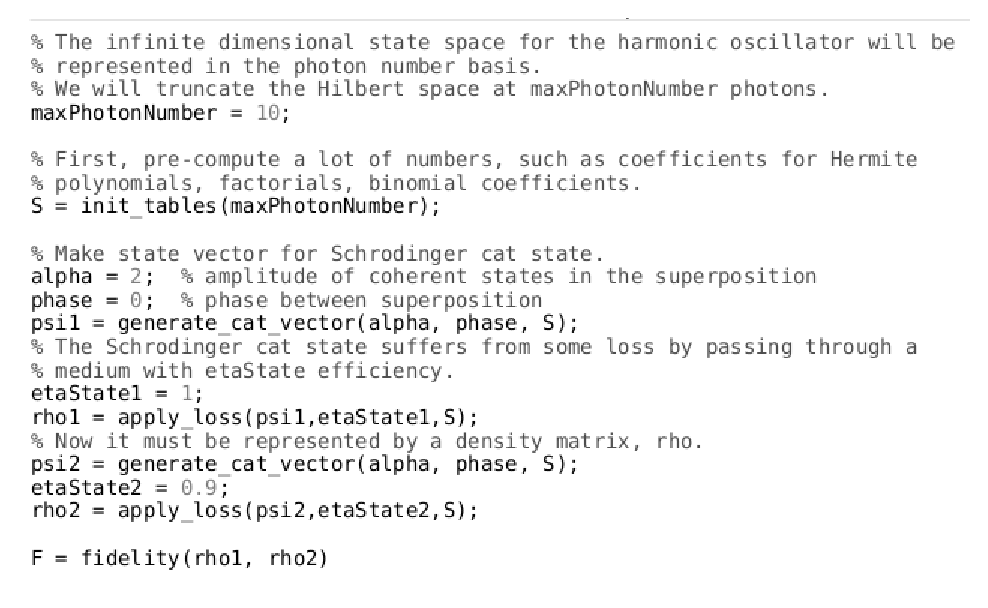
\includegraphics[width=0.5\textwidth]{fidelity.eps}
\end{figure}

In the example given, the fideliy is $F = 0.7171$.

\SGc{Some other tools that you might want to add: Phase evolution
  using \texttt{phase\_evolution.m} can help students visualize the
  harmonic oscillator dynamics.  Graphing quadrature probability
  distribution functions with \texttt{quadrature\_pdf.m}.  Calculating
  quadrature variances and comparing states' product of variances to
  the Heisenburg limit.  Calculating photon probability distributions
  and mean photon number.}

\section{Conclusion}
\label{conclusion}
The toolbox of computational routines described in this paper has been
proved useful for teaching quantum mechanics and quantum optics
courses. The lines of code developed for this toolbox facilitates the
visualization of quantum states using the Wigner quasi-probability
distibution, also called the Wigner function. \SG{Our code is
  available at ....}

\bibliographystyle{spphys}

\bibliography{teachingQO}

\end{document} 
